%%% LaTeX Template: Two column article
%%%
%%% Source: http://www.howtotex.com/
%%% Feel free to distribute this template, but please keep to referal to http://www.howtotex.com/ here.
%%% Date: February 2011

%%% Preamble
\documentclass[	DIV=calc,%
							paper=a4,%
							fontsize=12pt,%
							onecolumn]{scrartcl}	 					% KOMA-article class

\usepackage{lipsum}													% Package to create dummy text
\usepackage[brazil]{babel}										% English language/hyphenation
\usepackage[protrusion=true,expansion=true]{microtype}				% Better typography
\usepackage{amsmath,amsfonts,amsthm}					% Math packages
\usepackage[pdftex]{graphicx}									% Enable pdflatex
\usepackage[svgnames]{xcolor}									% Enabling colors by their 'svgnames'
\usepackage[hang, small,labelfont=bf,up,textfont=it,up]{caption}	% Custom captions under/above floats
\usepackage{epstopdf}												% Converts .eps to .pdf
\usepackage{subfig}													% Subfigures
\usepackage{booktabs}												% Nicer tables
\usepackage{fix-cm}													% Custom fontsizes
\usepackage[utf8]{inputenc}
\usepackage[top=2.5cm, bottom=2.5cm, left=2.5cm, right=2.5cm]{geometry}
\usepackage[ddmmyyyy]{datetime}
\addto\captionsenglish{%
	\renewcommand\tablename{Tabela}
	\renewcommand\figurename{Figura}
} 
 

 
%%% Custom sectioning (sectsty package)
\usepackage{sectsty}													% Custom sectioning (see below)
\allsectionsfont{%															% Change font of al section commands
	\usefont{OT1}{phv}{b}{n}%										% bch-b-n: CharterBT-Bold font
	}

\sectionfont{%																% Change font of \section command
	\usefont{OT1}{phv}{b}{n}%										% bch-b-n: CharterBT-Bold font
	}



%%% Headers and footers
\usepackage{fancyhdr}												% Needed to define custom headers/footers
	\pagestyle{fancy}														% Enabling the custom headers/footers
\usepackage{lastpage}	

% Header (empty)
\lhead{}
\chead{}
\rhead{}
% Footer (you may change this to your own needs)

%% ====================================
%% ====================================
%% mude o rodape  do projeto
%% ====================================
%% ====================================

\lfoot{\footnotesize \texttt{Cabeamento estruturado} \textbullet ~Modelo de projeto}


\cfoot{}
\rfoot{\footnotesize página \thepage\ de \pageref{LastPage}}	% "Page 1 of 2"
\renewcommand{\headrulewidth}{0.0pt}
\renewcommand{\footrulewidth}{0.4pt}



%%% Creating an initial of the very first character of the content
\usepackage{lettrine}
\newcommand{\initial}[1]{%
     \lettrine[lines=3,lhang=0.3,nindent=0em]{
     				\color{DarkGoldenrod}
     				{\textsf{#1}}}{}}



%%% Title, author and date metadata
\usepackage{titling}															% For custom titles

\newcommand{\HorRule}{\color{DarkGoldenrod}%			% Creating a horizontal rule
									  	\rule{\linewidth}{1pt}%
										}

\pretitle{\vspace{-30pt} \begin{flushleft} \HorRule 
				\fontsize{50}{50} \usefont{OT1}{phv}{b}{n} \color{DarkRed} \selectfont 
				}

%% ====================================
%% ====================================
%% mude o titulo  do projeto
%% ====================================
%% ====================================

\title{Modernização e Organização de Cabos Unimed-Foz}					% Title of your article goes here

%% ====================================



\posttitle{\par\end{flushleft}\vskip 0.5em}

\preauthor{\begin{flushleft}
					\large \lineskip 0.5em \usefont{OT1}{phv}{b}{sl} \color{DarkRed}}
\author{Jeverson Siqueira}  	% Author name goes here


\postauthor{\footnotesize \usefont{OT1}{phv}{m}{sl} \color{Black} 
					\\Universidade Tecnológica Federal do Paraná - Câmpus Cornélio Procópio 								% Institution of author
					\par\end{flushleft}\HorRule}

\date{}																				% No date




%%% Begin document
\begin{document}
\maketitle
\thispagestyle{fancy} 	
\thispagestyle{empty}		% Enabling the custom headers/footers for the first page 
% The first character should be within \initial{}




%% ====================================
%% ====================================
%% mude o resumo  do projeto
%% ====================================
%% ====================================
\initial{E}\textbf{
	Este projeto visa a modernização, organização e certificação dos cabos atuais no data center da Unimed Foz do Iguaçu, isso ira prover redução de erros na camada física, facilidade em encontrar erros na camada física, crescimento organizado, escalabilidade, segmentação modular da camada física e manutenção em setores. Todos os dados aqui levantados serão fictícios para a realização desse trabalho, mas será levantado como base alguns dados reais, que serão descritos no decorrer desse projeto. 
}

%% ====================================
\begin{figure}
	\centering
	
\includegraphics{utfpr}
\end{figure}

\vspace{3cm}
\centerline{\textit{\textbf{\today}}}





\clearpage
\renewcommand{\contentsname}{Sumário}
\tableofcontents
\clearpage

%% ====================================
%% ====================================
%% Inicio do texto
%% ====================================
%% ====================================
\section{Introdução}

A atual Unimed localizada no centro de Foz do Iguaçu conta com 40 colaboradores em sua sede administrativa, e no hospital conta com mais 100 colaboradores. Cada uma das Unimed possui seu próprio data center com isso iremos aplicar primeiramente na sede onde possui um parque de máquinas menores comparadas ao hospital. Atualmente na Unimed sede contamos com 45 equipamentos para uso dos funcionários, no data center contamos com um Storage de backup diário, um servidor mais completo para virtualizações onde nele conta com as virtualizações do LDAP (Lightweight Directory Access Protocol), servidor Web, Firewall e Proxy. As demais aplicações que os usuários usam são software normais do dia-a-dia como e-mail, edição de arquivos de textos e sistemas voltados para saúde etc. Esse documento será aplicado no data center para melhorar primeiro a sua estrutura, as demais equipamentos serão atualizados os cabos de rede, para assim manter um padrão adequados entre eles.

\subsection{Benefícios}
Os benefícios que teria após a execução desse projeto serias várias tais como: 

\begin{itemize}
	\item Redução de erros na camada física;
	\item facilidade em encontrar erros na camada física;
	\item crescimento organizado;
	\item escalabilidade;
	\item segmentação modular da camada física;
	\item manutenção em setores.
\end{itemize}
 
\subsection{Organizações Envolvidas}
A atual organização envolvida é a Unimed sede administrativa, ainda existe o Hospital que já é outro cenário tendo mais computadores e colaboradores, os servidores lotados no Unimed administrativo possui as mesmas funções do que no hospital, sendo uma AD, Proxy, Firewall e um para sistema de arquivos. No entanto não será levantado um cenário em comparação entre os dois. Talvez isso seja em algum outro trabalho futuro.


\section{Requisitos}\label{sec:Requisitos}
Os requisitos coletados para implantação levantados verificando as estrutura atual do data center podem ser visto na tabela \ref{tab:requisitos}.

\begin{table}[!htbp]
	\centering
	\begin{tabular}{|l|l|ll}
		\cline{1-2}
		\textbf{Componentes}        & \textbf{Qts.} &  &   \\
		\cline{1-2}
		Patch panel (furukawa GIGALAN CAT.6 de 24 portas) & 3    &  &   \\
		Switch gerenciável (Cisco 2960L ) & 2    &  &   \\
		Access Points 	   (Cisco Air-lap 1141n-a-k) & 4    &  &   \\
		Servidor Monitoramento SNMP 	   & 1    &  &   \\	
		Patch Cord Cat.6  1m	   & 72    &  &   \\
		Patch Cord Cat.6  5m	   & 72    &  &   \\
		\cline{1-2} 
	\end{tabular}
		\caption{Tabela para requisitos do projeto}\label{tab:requisitos}
\end{table}


\section{Usuários e Aplicativos}
A quantidade atual de usuário na Unimed sede são de 40 colaboradores, a estimativa de evolução é de pouco colaboradores devido as demandas da empresa, pensado nisso na seção \ref{sec:Requisitos} foram devidos mais estrutura do que atual, pensado já no crescimento de equipamentos e usuários na rede, assim como pontos de redes necessários. 

\subsection{Usuários}
	A seguir pode ser conferido na tabela \ref{tab:usuarios} a quantidade de usuários, juntamente com seus perfil de acesso:
	\begin{table}[!htbp]
		\centering
		\begin{tabular}{|l|l|ll} 
			\cline{1-2}
			\textbf{Usuários}                                  & \textbf{Perfil de acessos} &  &   \\ 
			\cline{1-2}
			Usuário Comuns                                     & 45                         &  &   \\
			Usuário Administradores                            & 2                          &  &   \\
			Usuários VPN                                       & 3                          &  &   \\
			Usuários Para Demais aplicações (Antivírus, Roots) & 5                          &  &   \\
			\cline{1-2}
		\end{tabular}
		\caption{Tabela com perfis de usuários}\label{tab:usuarios}
	\end{table}

\subsection{Aplicativos}
Aqui são demostrados as aplicações dos usuário e críticas do projeto, alguma aplicações são críticas dependendo de sua utilidades ou setor, por exemplo setores como financeiro e perícia médica devem serem alojados em Vlans específicas e manter uma certa prioridade em relação dos backup individuais de cada equipamento. 

\begin{table}[!htbp]
	\centering
	\resizebox{\textwidth}{!}{\begin{tabular}{|l|l|l|l} 
		\cline{1-3}
		\textbf{Setor} & \textbf{Nível de complexidade} & \textbf{Aplicações}                                                        &   \\ 
		\cline{1-3}
		RH             & Média                          & Aplicações de Cartão Ponto, E-mail e edição de textos~                     &   \\ 
		\cline{1-3}
		Liberação~     & Alta                           & Aplicações de liberações de exames, E-mail, edição de texto                &   \\
		\cline{1-3}
		SAC            & Baixa                          & Aplicações de texto, e-mail                                                &   \\
		\cline{1-3}
		Cadastro       & Média                          & Criação de contas e planos, E-mail, edição de textos                       &   \\
		\cline{1-3}
		Comercial      & Média                          & Software de Design e market, acesso a redes socias, e-mail edição de texto &   \\
		\cline{1-3}
		TI       	   & Alta                           & Gerenciamento de usuários, Datacenter, todo funcionamento dos softwares   &   \\
		\cline{1-3}
	\end{tabular}}
	\caption{Aplicações e nível de complexidade dos usuários}\label{tab:aplicacoes}
\end{table}


\section{Estrutura predial existente}
A estrutura da sala do data center junto com as distâncias dos cabos e servidores são descritas em imagens para o melhor entendimento do projeto, será apresentada a descrição junto com a topologia aplicada na sala.

\section{Planta Lógica - Elementos estruturados}

\subsection{Plano do Projeto}
A seguir será apresentada as imagens junto com a posição dos racks que irão conter os servidores, switch, patch panel, local da refrigeração e demais configurações.

\subsection{Desenho da Estrutura} 
O desenho da estrutura que se deseja montar para poder agrupar todos os equipamentos do data center pode ser observado na Figura \ref{fig:desenhoestrutura}

\begin{figure}[!htbp]
	\centering
	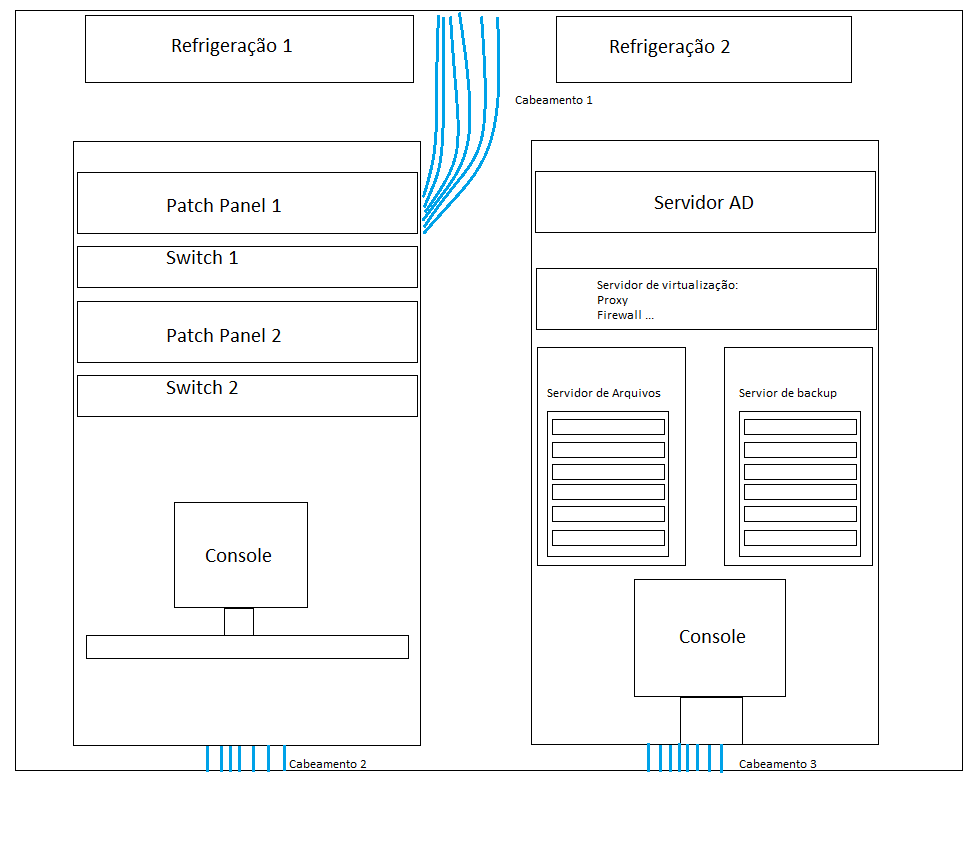
\includegraphics[width=\textwidth]{./imagens/datacenter.png}
	\caption{Exemplo de figura com escala horizontal}
	\label{fig:desenhoestrutura}
\end{figure}

	
\subsection{Topologia}
A topologia de redes física segundo \cite{forouzan2007} se refere à maneira pela qual uma rede é organizada fisicamente. Dois ou mais dispositivos se conectam a um link de comunicação; dois ou mais links formam uma topologia. Existe ainda o cenário de ser implementado uma topologia física e implantar uma topologia lógica diferente da Física. Na figura \ref{fig:tipos_topologias} pode ser visto alguns modelos de topologia, cada uma delas apresenta suas qualidades e defeitos, cabe a ao administrador definir qual melhor utilizar.

\begin{figure}[!htbp]
	\centering
	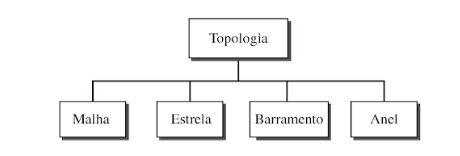
\includegraphics[width=\textwidth]{./imagens/tipos_topologia.png}
	\caption{Tipos de topologia}
	\cite{forouzan2007}
	\label{fig:tipos_topologias}
\end{figure}
 
\begin{figure}[!htbp]
 	\centering
 	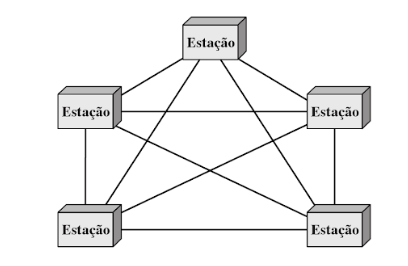
\includegraphics[width=\textwidth]{./imagens/malha.png}
 	\caption{Topologia Malha}
 	\cite{forouzan2007}
 	\label{fig:malha}
 \end{figure}

\begin{figure}[!htbp]
	\centering
	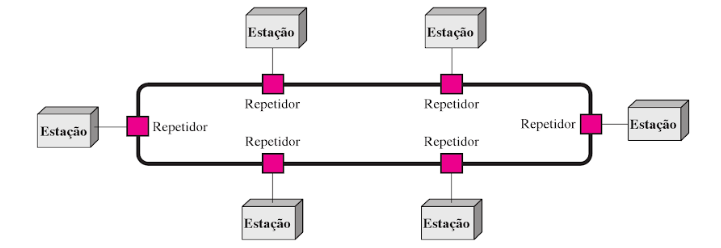
\includegraphics[width=\textwidth]{./imagens/anel.png}
	\caption{Topologia Anel}
	\cite{forouzan2007}
	\label{fig:anel}
\end{figure}
 
\begin{figure}[!htbp]
 	\centering
 	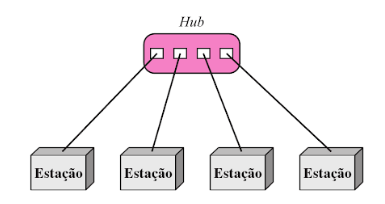
\includegraphics[width=\textwidth]{./imagens/estrela.png}
 	\caption{Topologia Estrela}
 	\cite{forouzan2007}
 	\label{fig:estrela}
 \end{figure}

\begin{figure}[!htbp]
	\centering
	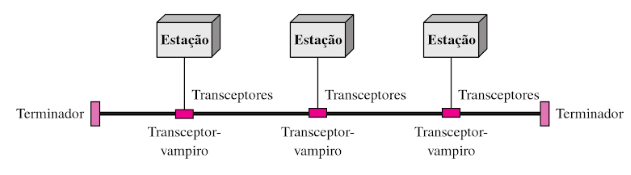
\includegraphics[width=\textwidth]{./imagens/barramento.png}
	\caption{Topologia Barramento}
	\cite{forouzan2007}
	\label{fig:barramento}
\end{figure}

De todas as topologias apresentada a mais ideal para o projeto seria topologia estrela conforme a Figura \ref{fig:estrela}. Segundo \cite{forouzan2007} a topologia em estrela cada dispositivo tem seu link ponto a ponto dedicado ligando apenas com o controlador central, em geral pode ser um Hub ou Switch. Os dispositivos não são ligados diretamente entre si. Diferentemente de uma topologia em malha, uma topologia em estrela não permite tráfego direto entre cada dispositivos. O Controlador atua como uma central telefônica: se um dispositivo quiser enviar dados para outro dispositivo, ele deve enviar ps dados primeiramente ao controlador que, então, os retransmite ao outro dispositivo. Em nosso cenário conforme descrito na Seção \ref{sec:Requisitos} o nosso controlado central será um Switch Cisco 2960L.
Esse Switch tem como as seguintes características são comutadores Gigabit Ethernet fixo e gerenciados de forma inteligente que fornecem comutadores de acesso de classe empresarial para filias, aplicativos "out-of-the-wiring closete" e implantações críticas de Internet das Coisas (Iot). Os Catalyst 2960-L Smart Managed Switches são switches seguros, confiáveis e de nível empresárias criados para implantações em pequenos escritórios. Esses switches podem ser configurados e gerenciados por meio de uma interface da Web on-box, permitindo aos clientes uma maneira rápida e confiável de colocar em funcionamento uma pequena filial ou uma rede de escritórios em poucos minutos. Esses switches também apresentam suporte CLI limitado para solução de problemas e monitoramento. Sendo ainda totalmente gerenciados que oferecem recursos avançados de Camada 2 e 3 básica, bem como energia Power Over Ethernet Plus (PoE +), oferecendo segurança de rede aprimorada, confiabilidade de rede e eficiência operacional. 
 	
\subsection{Encaminhamento}
Eletrodutos, calhas, e qualquer material em que os cabos serão alojados/alocados.

\subsection{Identificação dos cabos}
Explique como os cabos serão identificados em seu projeto. Coloque uma relação dos cabos instalados e identificados.

\section{Implantação}
Estabeleça um cronograma de implantação:
Remoção de equipamentos existentes (destino para descarte), instalação dos condutores, instalação dos cabos, 
identificação dos cabos, montagem dos racks, certificação, etc... Crie atividades e estabeleça o tempo de execução. Se for um projeto real, indique também quais os responsáveis pela execução do projeto e de cada uma das etapas.

Defina marcas (e padrões) e fornecedores se for o caso. Atenção a contratados e subcontratados para a realização das atividades. Estabeleça a responsabilidade de execução da atividade e também da validação dela.

Utilize algum software para gerear o cronograma. Excel,etc. O fundamental é dividir em etapas, descrever e estimar o tempo de cada uma delas.

Segue uma relação de ferramentas:
http://asana.com/, 
https://trello.com/, 
http://www.ganttproject.biz/, 
http://www.orangescrum.org/. 

\section{Plano de certificação}
Quais seriam as etapas para a certificação? 
Quais os locais e horários para execução da certificação na rede? Toda rede será certificada?
Como os testes seriam executados?
Quais relatórios de certificação serão (ou deveriam ser) entregues? 

\section{Plano de manutenção}

Revisões periódicas na rede, emissão de certificados para novos pontos.

\subsection{Plano de expansão}
Existe um plano de expansão? Quantos novos pontos poderão ser acrecidos na rede, antes de migração de equipamentos na camada 2? Se houver expansão, quais equipamentos deverão ser direcionados para as estremidades da rede? 

\section{Risco}
Enumerar e explicar os riscos do projeto.

\section{Orçamento}
Crie uma relação de orçamentos baseado na seções anteriores.

\section{Recomendações}
Observações e recomendações para o cliente.

\section{Referências bibliográficas}
Utilize o mendley, o jabref ou diretamente o bibtex para gerenciar suas referências biliográficas. As referências são criadas automaticamente de acordo com o uso no texto.

Exemplo: Redes de computadores, segundo \cite{t2013} é considerada..... Já \cite{kurose2010} apresenta uma versão...

Analisando os pressupostos de \cite{ref3} e \cite{ref4} concluimos que....


\renewcommand\refname{} %%Referências bibliográficas}  
\bibliographystyle{ieeetr}
\bibliography{referencias}  

%% ***********************************************************************
%% === remover daqui =====================================================
%% ***********************************************************************
=================================================
\section{Elementos textuais - Alguns exemplos}

Esta seção apresenta exemplos de elementos textuais. \textbf{Remova-a da versão final do texto}.


\subsection{Colocar elementos em itens}

Texto antes da lista

\begin{itemize}
	\item First item in a list 
	\item Second item in a list 
	\item Third item in a list
\end{itemize}

\subsubsection{Uma subseção de terceiro nivel}

Exemplo de uma subseção

\subsection{Tabelas}

Utilize o site http://www.tablesgenerator.com/ para elaborar as tabelas de seu trabalho.
Para adicionar uma tabela utilize: a tag input, passando o arquivo da tabela como parametro

\begin{table}[h!] % coloque h! para forcar a posicao
\centering
\caption{Modifique a legenda e crie um label}
\label{tab2} %com este label vc faz referencia no texto
\begin{tabular}{|l|l|l|l|l|}
\hline
\multicolumn{1}{|c|}{\textbf{Este é um exemplo de tabela}} & \multicolumn{2}{c|}{\textbf{C1}} & \multicolumn{2}{c|}{\textbf{C2}} \\ \hline
Você pode criar a tabela no excel                          & 1              & 2               & 3               & 4              \\ \hline
Exportar para CSV                                          & 5              & 6               & 7               & 8              \\ \hline
E importar no Table Generator                              & 9              & 10              &                 &                \\ \hline
\multicolumn{5}{|c|}{\textit{Gere o tex, e adicione em seu arquivo}}                                                             \\ \hline
\end{tabular}
\end{table}

Dentro do arquivo você deve definir o label e pode utilizá-lo para referenciar. Exemplo:
Na tab \ref{tab2} temos a relação de ....


Você também pode modificar a tabela manualmente, incluindo, por exemplo h! dentro de sua definição. Veja no exemplo tab2.tex

\subsection{Figuras}

As figuras podem ser no formato PDF, JPG, PNG. Você pode referenciá-las da mesma maneira que tabelas. Exemplo: A figura \ref{fig1} apresenta.....

Não se preocupe o local em que a figura será renderizada em seu texto. Preocupe-se em criar referência para ela, ou seja, toda figura e tabela deve conter pelo menos uma referência no texto.

\begin{figure}
\centering
\includegraphics[width=\textwidth]{fig1}
\caption{Exemplo de figura com escala horizontal}
\label{fig1}
\end{figure}


\begin{figure}
	\centering
	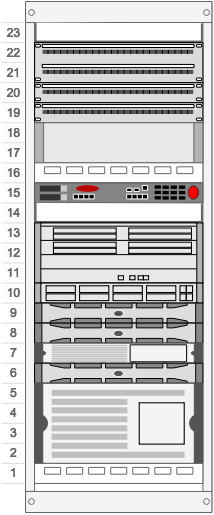
\includegraphics[]{fig2}
	\caption{Exemplo de figura sem escala}
	\label{fig2}
\end{figure}

Você pode rotacionar figuras também. Para isso utilize o parâmetro angle=-90. Repare que a escala da figura foi modificada pelo parametro height. Você também pode utilizar scale

\begin{figure}
	\centering
	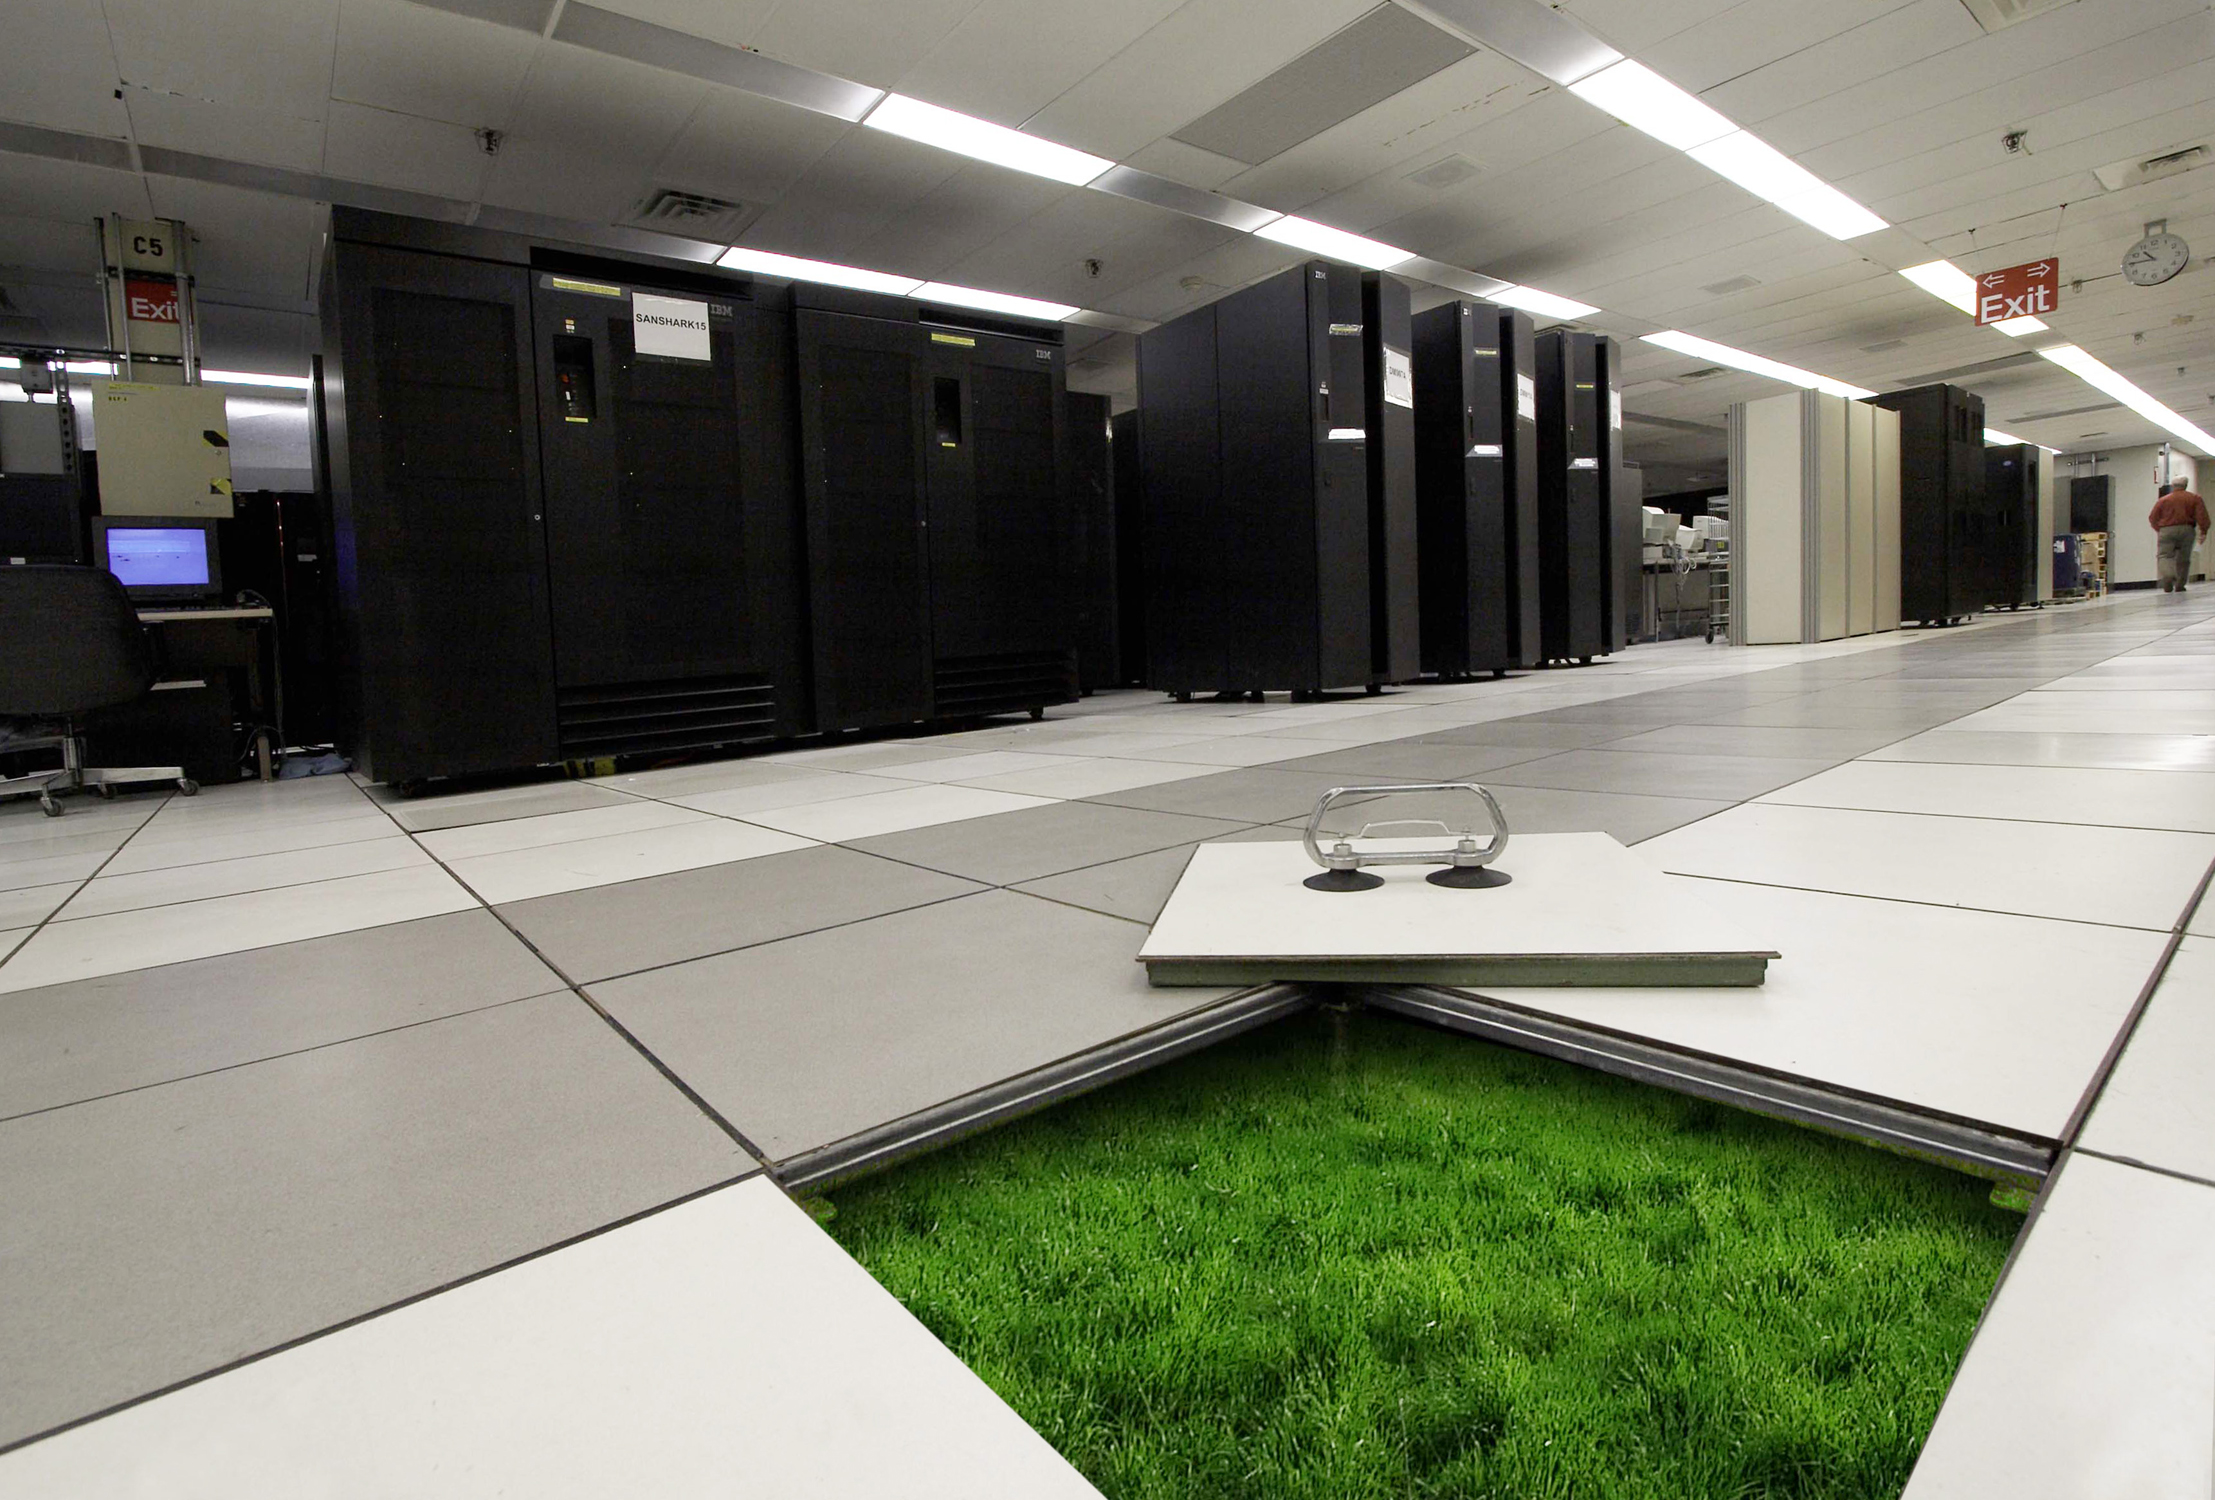
\includegraphics[height=\textwidth,angle=-90]{fig3}
	\caption{Exemplo de figura rotacionada}
	\label{fig3}
\end{figure}


%% ***********************************************************************
%% === ate aqui    =====  ================================================
%% ***********************************************************************

\end{document}